
\documentclass[12pt]{article}
\usepackage{geometry}
\usepackage{listings}
\usepackage{float}
\usepackage{xcolor}
\usepackage{graphicx}
\usepackage{booktabs}
\usepackage{marginnote}
\usepackage{caption}
\usepackage{multicol}
\usepackage{subfig}
\usepackage{setspace}
\definecolor{codegreen}{rgb}{0,0.6,0}
\definecolor{codegray}{rgb}{0.5,0.5,0.5}
\definecolor{codepurple}{rgb}{0.58,0,0.82}
\definecolor{backcolour}{rgb}{0.95,0.95,0.92}
\lstdefinestyle{mystyle}{
  backgroundcolor=\color{backcolour},  commentstyle=\color{codegreen},
  keywordstyle=\color{magenta},
  numberstyle=\tiny\color{codegray},
  stringstyle=\color{codepurple},
  basicstyle=\ttfamily\footnotesize,
  breakatwhitespace=false,
  breaklines=true,
  captionpos=b,
  keepspaces=true,
  numbers=left,
  numbersep=5pt,
  showspaces=false,
  showstringspaces=false,
  showtabs=false,
  tabsize=2
}
%"mystyle" code listing set
\lstset{style=mystyle}
%\lstset{basicstyle=\ttfamily\footnotesize,breaklines=true}

\geometry{
  a4paper,
  total={170mm,257mm},
  left=20mm,
  top=20mm,
  }

\usepackage[breaklinks]{hyperref}
% Setup de hiperenlaces
\hypersetup{
  colorlinks=true,
  linkcolor=blue,
  filecolor=magenta,
  urlcolor=cyan,
  pdftitle={Examen - Juego NDS - Jess Jimnez Montero},
  citecolor = green
}

\usepackage{url}

%\usepackage{fontspec}
%\setmainfont{AT-NameSansText}[
%  Path=./NameSansStatic/,
%  Extension = .otf,
%  UprightFont=*-Regular,
%  BoldFont=*-Bold,
%  ItalicFont=*-RegularItalic,
%  BoldItalicFont=*-BoldItalic,
%  Numbers = OldStyle
%]
%
%\setmonofont{ATNameMono}[
%  Path=./NameMonoStatic/,
%  Extension = .otf,
%  UprightFont=*-Regular,
%  BoldFont=*-Bold,
%  ItalicFont=*-RegularItalic,
%  BoldItalicFont=*-BoldItalic
%]

\usepackage{fancyhdr}
\fancypagestyle{plain}{% the preset of fancyhdr
  \fancyhf{} % clear all header and footer fields
  \fancyfoot[R]{
\includegraphics[width=2cm]{Imagenes/uji.jpg}}
  %\fancyfoot[L]{\thedate}
  \fancyhead[L]{Videojuego creado en Unity: \textunderscore deadSet}
  \fancyhead[R]{\theauthor}}

\usepackage[backend=biber]{biblatex}
\addbibresource{referencias.bib}
\usepackage{notoccite}
\renewcommand{\figurename}{\textbf{Figura.}}
\renewcommand{\tablename}{\textbf{Tabla.}}
\renewcommand*{\contentsname}{Tabla de contenidos}
\renewcommand{\listfigurename}{Lista de imgenes}
% \setcounter{secnumdepth}{5}
% \setcounter{tocdepth}{4}


%---------------------------------
%DOCUMENTO
%---------------------------------
\begin{document}
\nocite{namesans_about}
\nocite{namesans}
\nocite{namemono}
\nocite{seriouscode-gmbh-2022}
\nocite{carbon}
\nocite{fnaf_ai}
\nocite{fnaf_assets}
\nocite{fnaf_decomp}


  \begin{titlepage}
    \begin{center}
      \vspace{5cm}

      {\Huge \textbf{Juego NDS: \\
      Five Night's At Freedy's}}

      \vspace{2cm}

      
\includegraphics[width = \textwidth]{Imagenes/uji.jpg}

      \vspace{2cm}

      {\Large \textit{Jess Jimnez Montero}}\\
      \vspace{1cm}
      {\Large \textit{VJ1214 - Consolas y Dispositivos de Videojuegos}}\\

      \vspace{2cm}
    \end{center}
  \end{titlepage}

  \newpage


\spacing{1.15}
\begin{abstract}
  Este juego es un \textit{"demake"} \footnote{De WikiPedia: Un demake es una reimaginacin de un videojuego en una plataforma ms antigua de la original; o una que convierte a este a un estilo grfico u otorga una jugabilidad ms antigua.} del popular juego de PC: \textit{Five Night's At Freedy's}. La idea es realizar una adaptacin de FNAF a la Nintendo DS, tomando ventaja de las funciones que caracterizan a la NDS como la pantalla tctil y la portabilidad. Todo el juego est pensando para ejecutarse en una NDS real.
\end{abstract}
\newpage

% NDICE
\tableofcontents
\newpage

\listoffigures
\newpage


\section{Propuesta de juego}
  Five Night's at Freddy's, es un juego de supervivencia en el que debes sobrevivir 6 horas en el local de Freddy's Pizzeria como guarda de seguridad. Tu objetivo para mantenerte a salvo es comprobar las cmaras para seguir el rastro de los animatrnicos, cerrar las puertas para evitar que entren en tu oficina y usar la linterna para comprobar si hay alguno en el pasillo. Si alguno de los animatrnicos entra en tu oficina, pierdes la partida y reinicias la noche actual.\\

  La idea de llevar este juego a la NDS es que su jugabilidad casa fenomenalmente con cmo funciona la consola. Todo el juego se juega con el ratn en su versin original, as que, la jugabilidad se traduce naturalmente a la propia NDS.

  En el documento se referir al juego realizado en la NDS como demake para distinguirlo del juego original.

\newpage
\section{Jugabilidad y mecnicas}
  En esta seccin se explican en profundidad las mecnicas del juego desde el punto de vista del jugador, el resumen tcnico se pueden encontrar en la seccin \ref{how}.

  \subsection{Supervivencia}

    En pocas palabras, el jugador debe aguantar desde la 12AM hasta las 6AM, en la que los animatrnicos dejan de funcionar y se considera que el jugador ha ganado. Por trminos de jugabilidad, en el juego original son alrededor de 9 minutos (cada hora son 90 segundos de tiempo real), y en el demake 5 minutos (con cada hora siendo 60 segundos en el reloj de la NDS).

  \subsection{Defensas del jugador}
    El jugador se dispone en una sala de guarda de seguridad en la que dispone de dos entradas, una a su izquierda y otra a su derecha.

    \begin{figure}[!h]
      \begin{minipage}[c]{0.3\linewidth}
        \centering
        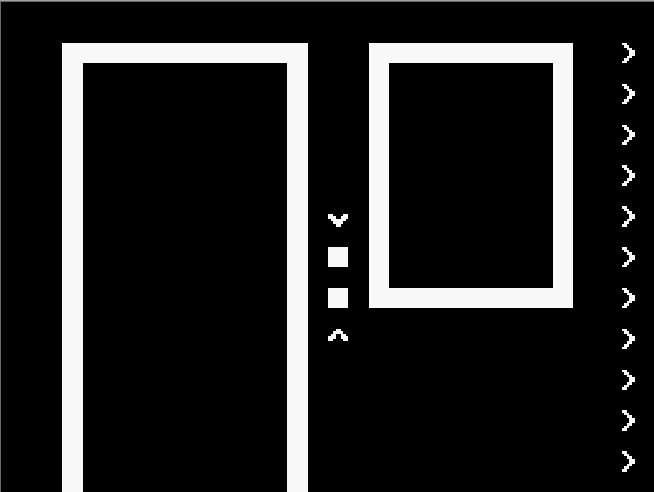
\includegraphics[width=\linewidth]{Imagenes/leftRoom.png}
        \caption{Vista de la puerta izquierda}
      \end{minipage}\:
      \begin{minipage}[c]{0.3\linewidth}
        \centering
        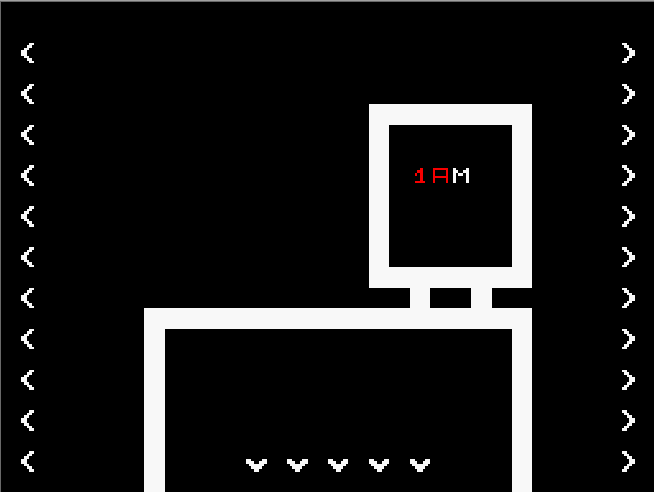
\includegraphics[width=\linewidth]{Imagenes/centerRoom.png}
        \caption{Vista central de la habitacin}
      \end{minipage}\:
      \begin{minipage}[c]{0.3\linewidth}
        \centering
        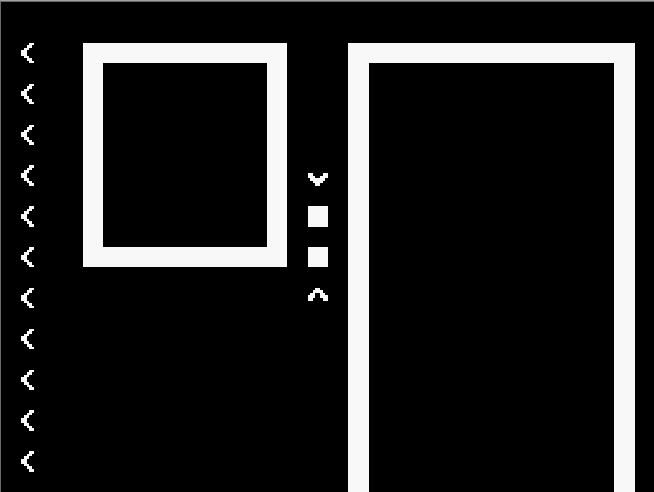
\includegraphics[width=\linewidth]{Imagenes/rightRoom.png}
        \caption{Vista derecha de la habitacin}
      \end{minipage}
    \end{figure}

    En cada una de las pantallas se dispone de una accin diferente, con las puertas pudiendo abrirlas y cerrarlas segn haya o no un animatrnico acechando justo afuera de la habitacin. Si estas se cierran antes de que el animatrnico pueda pasar, a este se le impide entrar.

    En la parte central se puede acceder al panel de cmaras:

    \begin{figure}[H]
      \centering
      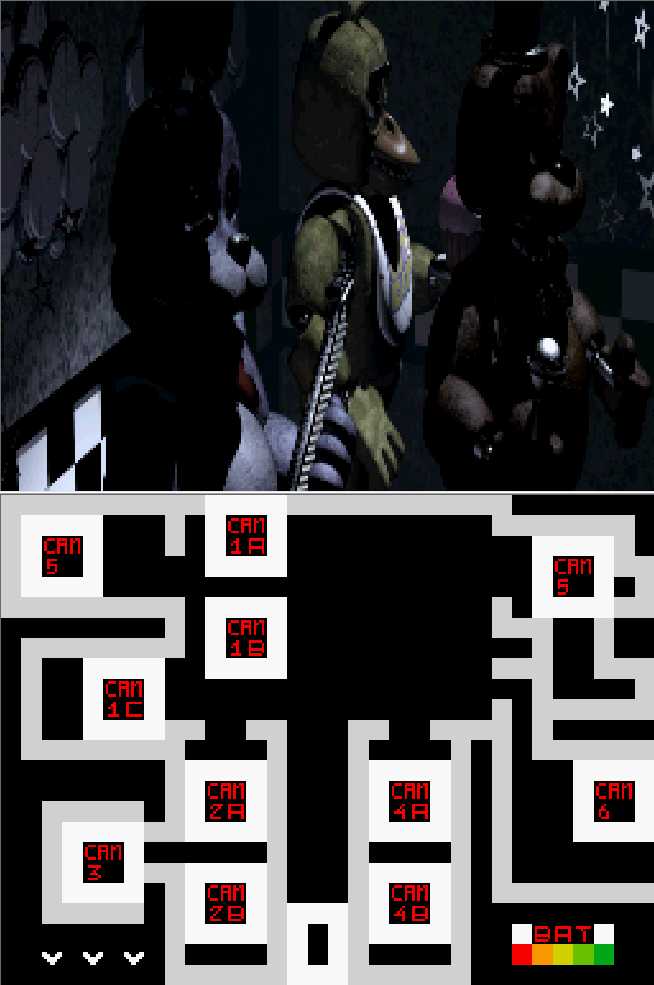
\includegraphics[width=0.75\linewidth]{Imagenes/camera}
      \caption[]{Panel de cmaras}
      \label{fig:camera}
    \end{figure}

    El cual permite vigilar los movimientos de los animatrnicos y mantener una idea de su recorrido y posiciones para saber cundo cerrar las puertas; ya que, como se puede ver en la esquina inferior izquierda, el jugador dispone de una cantidad de energa limitada que si llega a cero, se considera un game over.

    La batera es el nico recurso que el jugador debe manejar, con la batera agotndose progresivamente durante la noche; y agotndose algo ms rpido si el jugador mira las cmaras.

  \subsection{Enemigos: los animatrnicos}

    Los enemigos son animatrnicos robticos posedos, cuyo objetivo es introducir al jugador en un traje animatrnico debido a que un fallo de su programacin les hace creer que, por alguna razn, el personaje que controla el jugador es un endoesqueleto sin el disfraz; por lo que su objetivo es volver a introducir al personaje dentro de uno, con consecuencias nefastas.\footnote{Este es un resumen del propsito de los animatrnicos, el verdadero propsito es muy complicado y la historia de FNAF muy extensa, adems de que no es el objetivo de este documento explicar la historia del juego.}

    \subsubsection{Bonnie y Chica}
      Ambos funcionan de maneras similares, cada cierto tiempo, los animatrnicos se mueven de posicin acercndose lentamente a la sala de seguridad. Para detenerlos, cuando estn en la puerta y sean visibles desde la sala de seguridad (no las cmaras), se debe cerrar la puerta respectiva y esperar a que se vayan; representado de tal manera de que vuelven al estrado donde se encontraban en un primer lugar.

      \begin{figure}[!h]
        \begin{minipage}[c]{0.4\linewidth}
          \centering
          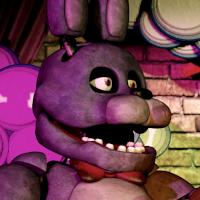
\includegraphics[width=0.75\linewidth]{Imagenes/bonno.png}
          \caption{Foto de Bonnie}
        \end{minipage}\:
        \begin{minipage}[c]{0.4\linewidth}
          \centering
          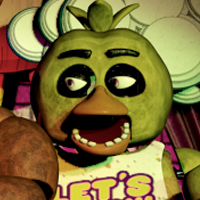
\includegraphics[width=0.75\linewidth]{Imagenes/chica.png}
          \caption{Foto de Chica}
        \end{minipage}\:
      \end{figure}


    \subsubsection{Foxy}
      Foxy funciona de manera parecida a los dos anteriores, cada cierto tiempo se mueve, pero en la misma cmara. Foxy funciona mediante estados, cada vez saliendo ms de su carpa hasta que llega su momento de atacar. Cuando llega a este estado, Foxy comenzar a correr hacia la sala de seguridad, teniendo que el jugador cerrar la puerta antes de que llegue.
      Esto har que el porcentaje de la batera baje un poco para evitar que entre.

      Otra manera de detener su progreso es mirndolo, lo que har que no pueda cambiar de fase mientras lo ests observando.
        \begin{figure}[H]
          \centering
          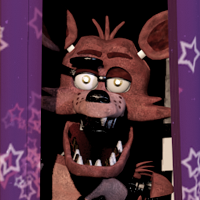
\includegraphics[width=0.35\linewidth]{Imagenes/foxy}
          \caption{Foto de Foxy}
          \label{fig:foxy}
        \end{figure}

\newpage
\section{Cmo se ha creado el juego? \label{how}}
  \subsection{Grficos}
    El juego toma ventaja de la NDS al mximo, aprovechando la ventaja de tener dos pantallas.
    La opcin ms lgica era implementar dos sistemas grficos, uno de teselas y un framebuffer.

    Las pantallas se configur el motor MAIN a dibujar la pantalla con LCD debido a que el motor sub no usar un framebuffer para mostrar la pantalla. El segundo motor dibujaba las teselas.
    \begin{figure}[H]
      \centering
      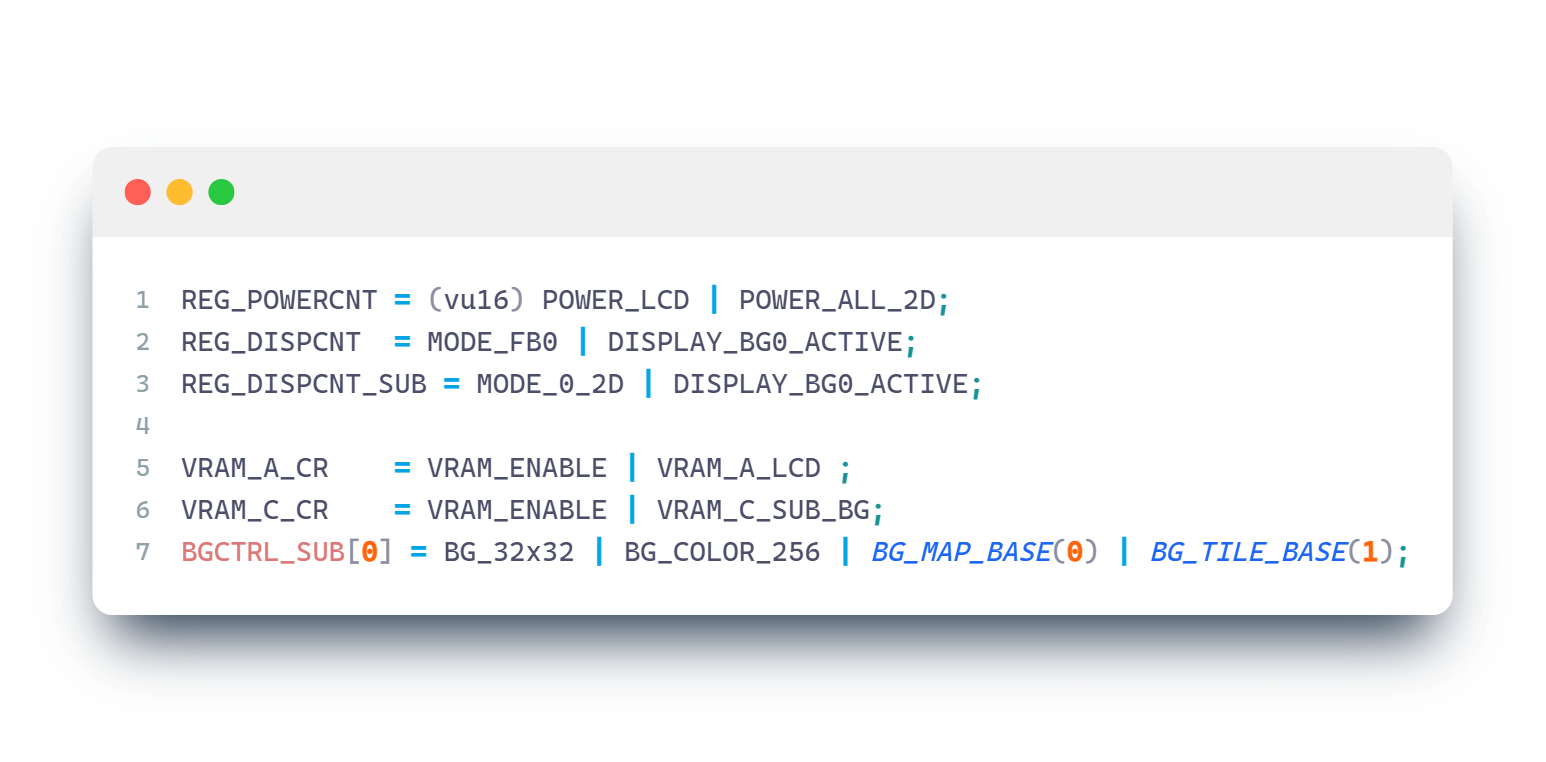
\includegraphics[width=\linewidth]{Imagenes/pantallas.png}
      \caption{Cdigo usado para configurar las pantallas}
      \label{fig:screen}
    \end{figure}

    Y para incluir todas estas teselas, se ide con ayuda de Microsoft Copilot \cite{copilot} una solucin para simplificar la copia de teselas en RAM:

    \begin{figure}[H]
      \centering
      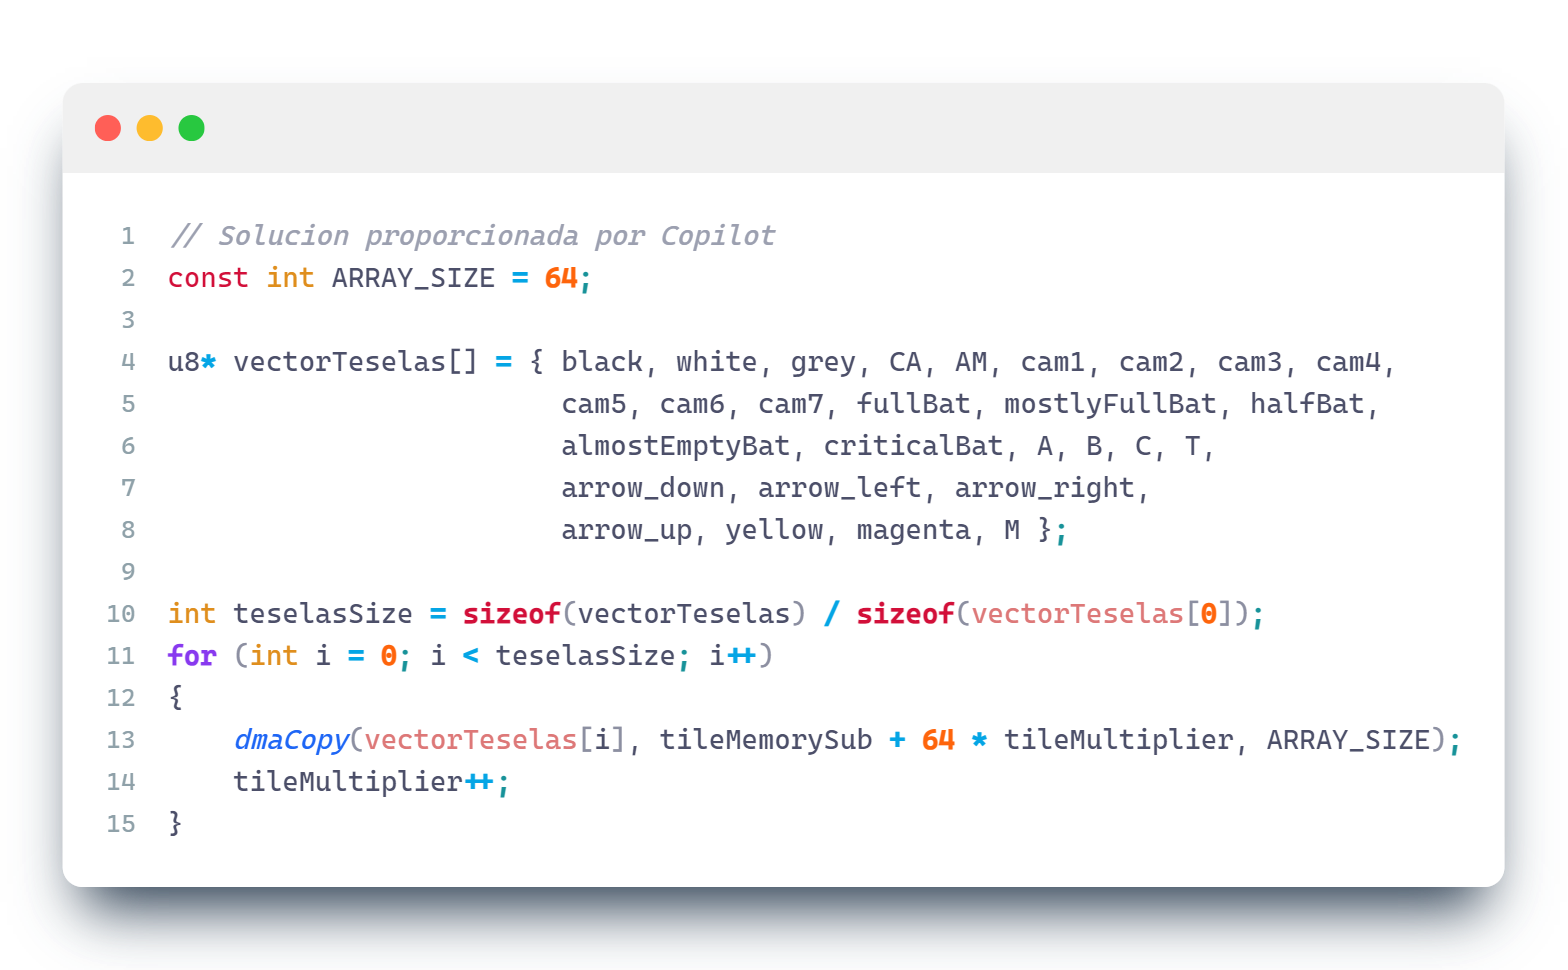
\includegraphics[width=0.75\linewidth]{Imagenes/teselas}
      \caption{Funcin de copia de teselas}
      \label{fig:teselas}
    \end{figure}

    Primero se define una constante que contiene el tamao de las teselas, luego se declara un vector de variable de 8bits sin signo y se almacenan todas las teselas. \\

    Con \texttt{teselasSize} se hace el clculo del tamao del array con \texttt{sizeof} aunque debido a que esto se proporciona en bytes, se divide entre el tamao del primer elemento del array y proporciona el nmero de elementos en el array. \\

    \texttt{tileMultiplier} simplemente hace el trabajo de en vez de poner +64, +128, se multiplica el 64 que es fijo, por el nmero que va constantemente incrementando.\\

    Despus con el bucle se usa el comando \texttt{dmaCopy()} para hacer la copia, intercambiando los valores introducidos a mano por variables. \\

    Las imgenes se copian en memoria en \textit{runtime}, cada pasada del bucle Update() se llama a una clase llamada \texttt{GameRenderer}, la dispone de varios mtodos que se encarga de redibujar la pantalla cada frame. Adems, cada mtodo dispone de las variables que se encuentran en \texttt{main.cpp} y en \texttt{GameRenderer}; pasadas como parmetro. \\

    \texttt{GameRenderer::Render()} se encarga de redibujar las teselas del motor SUB mediante un switch-case, que dependiendo de la posicion del jugador y si est mirando cmaras, se copia con un bucle las teselas a la memoria.


    \begin{figure}[H]
      \centering
      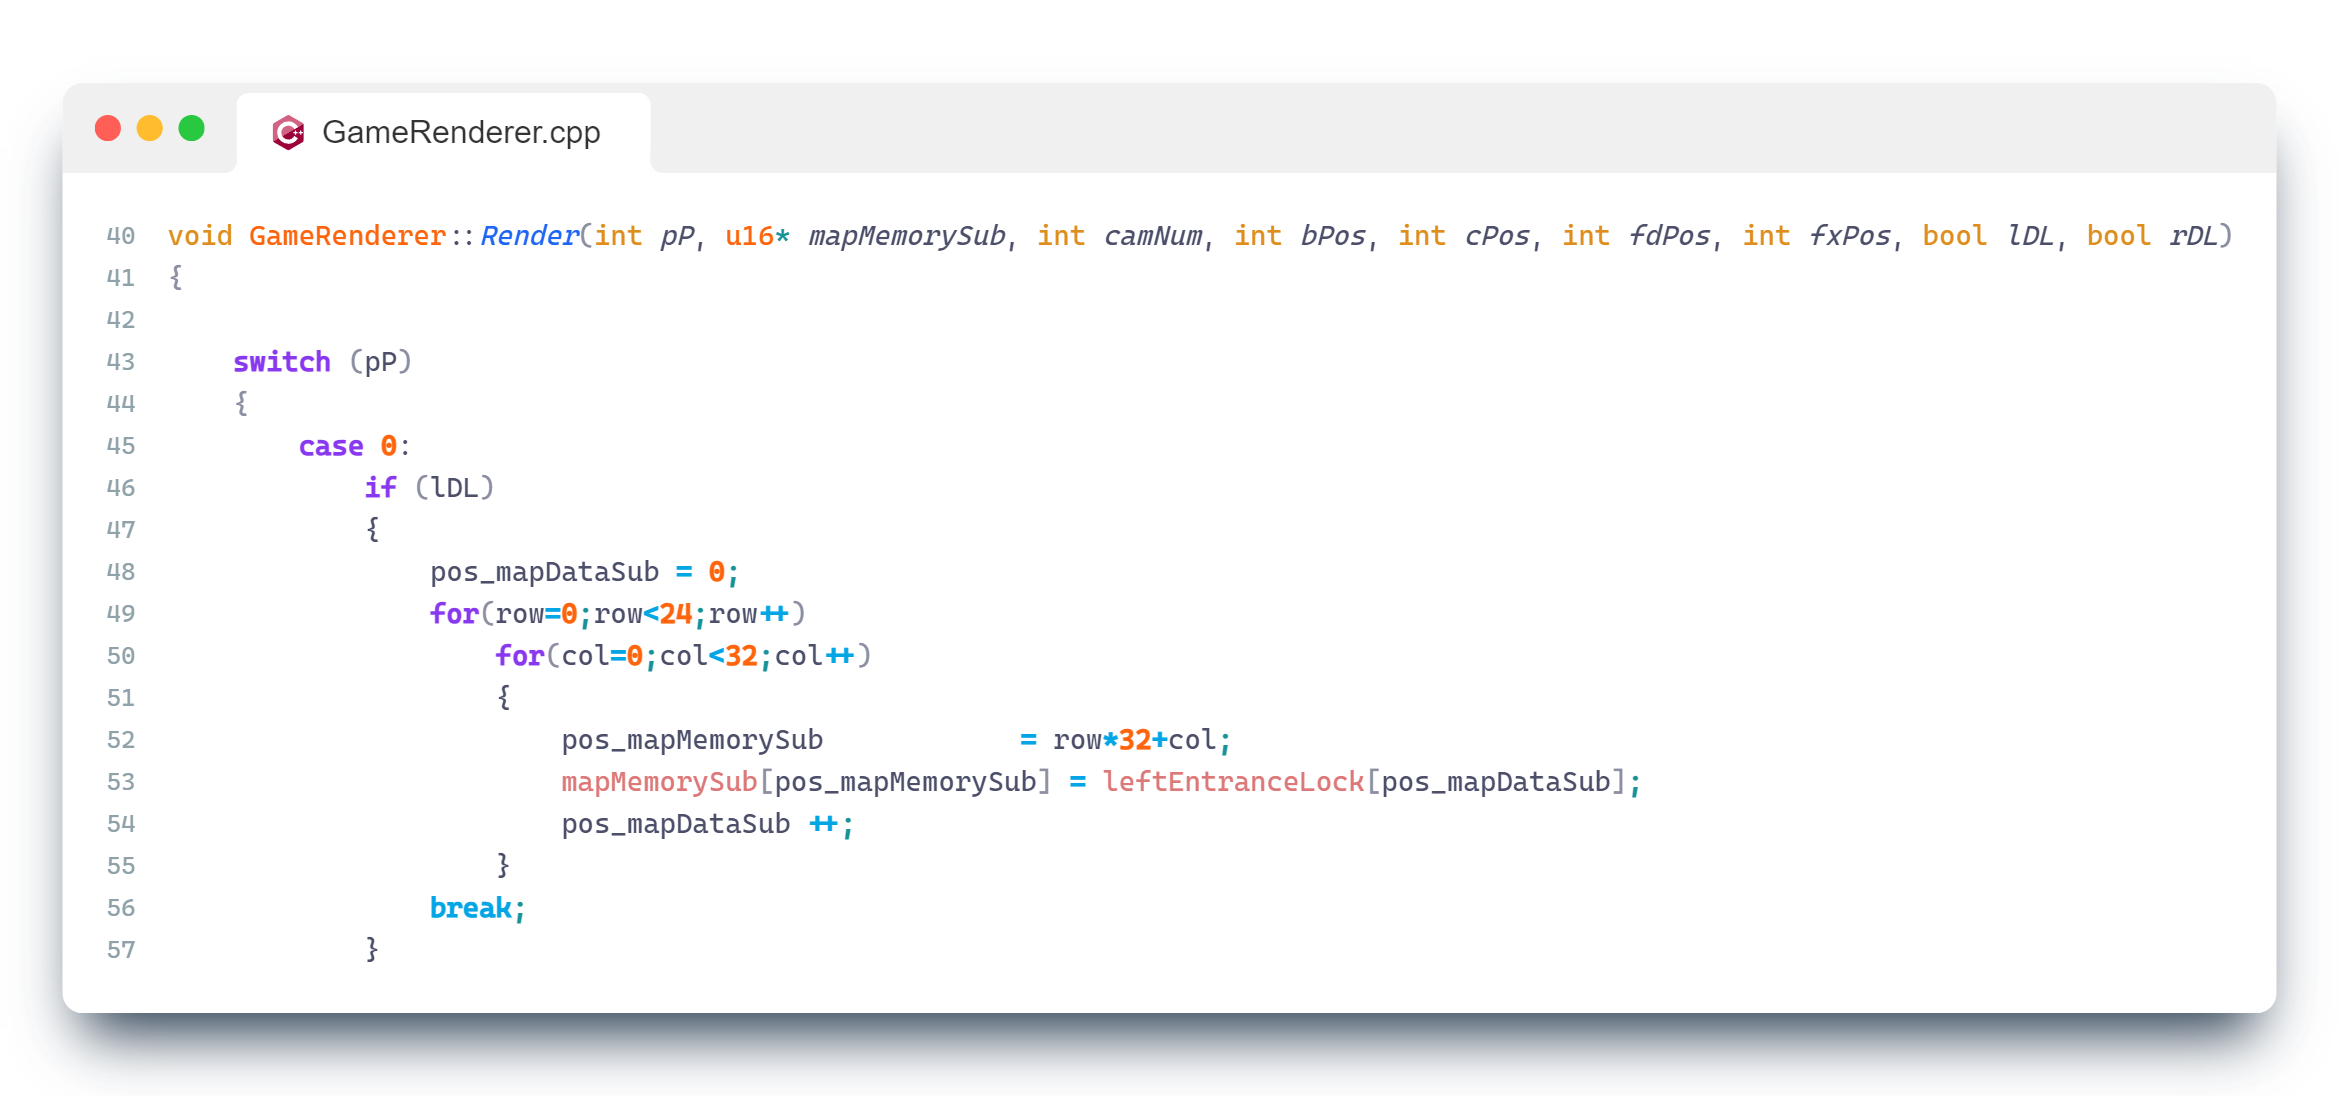
\includegraphics[width=0.75\linewidth]{Imagenes/GameRenderer-Render}
      \caption{Extracto de cdigo de Render}
      \label{fig:gamerenderer-render}
    \end{figure}


    Y las imgenes se deciden cul poner con condicionales:
    \begin{figure}[H]
      \centering
      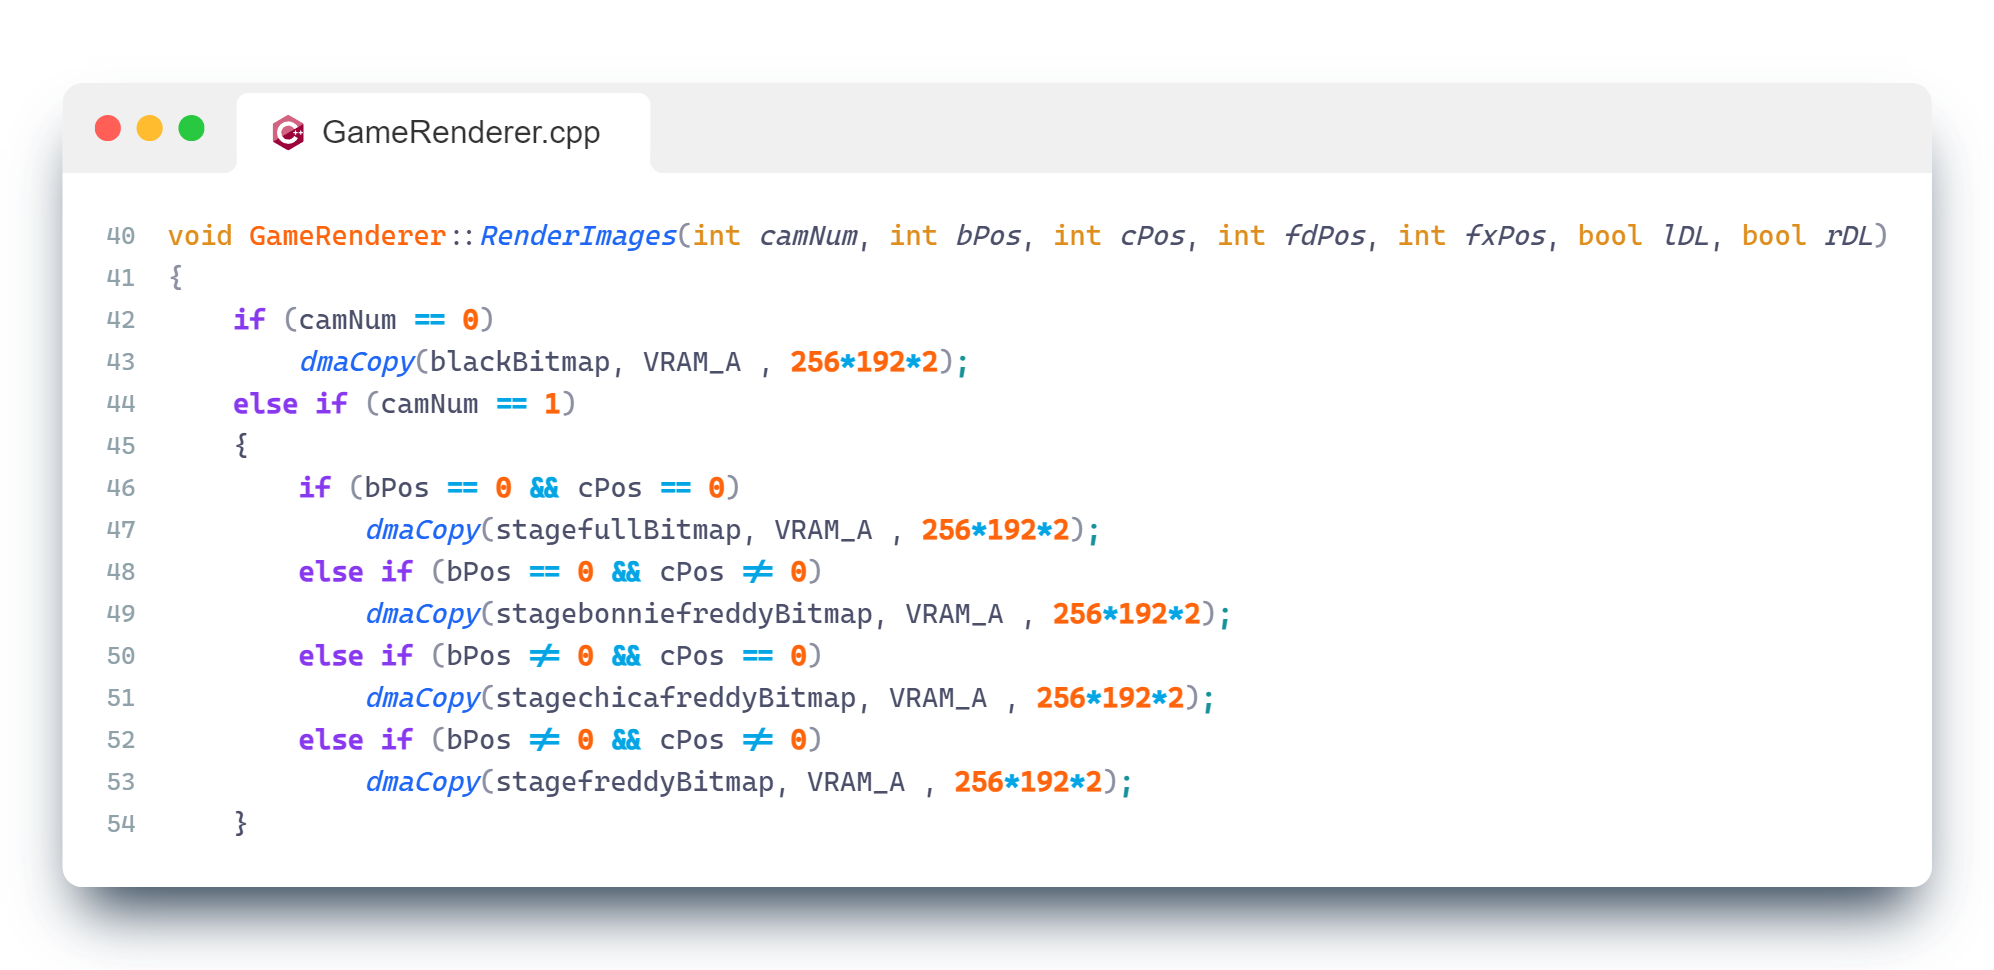
\includegraphics[width=0.75\linewidth]{Imagenes/gameRenderer-RenderImages}
      \caption{Extracto de cdigo de RenderImages}
      \label{fig:gamerenderer-renderimages}
    \end{figure}

  \subsubsection{Acciones del jugador}
    Los controles se realizaron mediante el uso de \texttt{keysDown() y keysHeld()} para simplificar el proceso de introducir los controles.

    Los controles se deciden cules estn activos y que se puede hacer segn el \texttt{playerPosition}. Por ejemplo, si \texttt{pP} no est en 3, significa que no est mirando las cmaras y puede moverse izquierda y derecha.

    Adems, al probar el juego en la NDS, se comprob que era muy incmodo cambiar entre las cmaras mediante toques, as se cambi el sistema para poder cambiar entre cmara manteniendo el lpiz.

    El juego tambin puede jugarse de forma parcial con botones y el lpiz, siendo este necesario para cambiar entre cmara como se ha mencionado antes.

  \subsection{IA y temporizadores}
    Sera mentira decir que no todo, pero casi todo el juego se mueve mediante temporizadores y todo se calcula mediante un temporizador global; la IA se mueve segn los segundos que hayan pasado; dispones de un nmero limitado de segundos para defenderte de Foxy; etc...

    La mayora de las acciones necesarias con temporizadores se manejan desde el \texttt{main.cpp} debido a que era ms fcil gestionar desde el Update() todo lo relacionado con los temporizadores y la:
    \subsubsection{Los animatrnicos y la IA}
      Al principio de la noche, el jugador obtiene un perodo de gracia en que los animatrnicos estn deshabilitados, dejando a este acostumbrarse un poco a los controles; adems de hacer el juego un poco ms amigable para el jugador.\\

      Cuando este perodo de gracia se termina, empiezan a moverse los animatrnicos segn un patrn, decisiones aleatorias.
      Los animatrnicos tienen un nivel de dificultad, que empieza en 0 y termina en 20; la mecnica de movimiento funciona tirando un dado, es decir, se obtiene un nmero aleatorio y se compara con el nivel de dificultad del animatrnico; resumidamente:

      $$if (randomNum <= nivelDificultad = moverse)$$
      \begin{figure}[H]
        \centering
        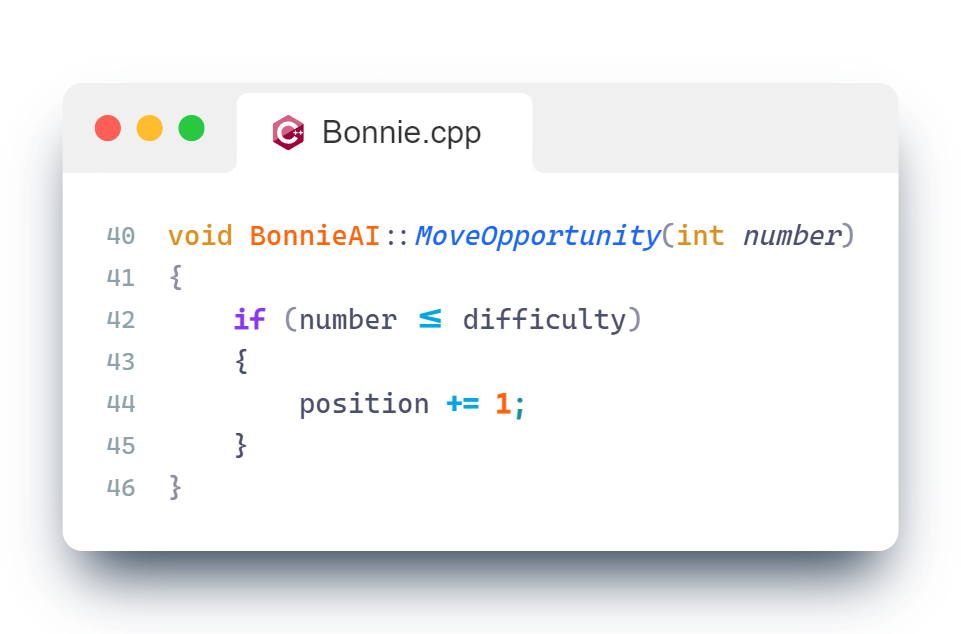
\includegraphics[width=0.75\linewidth]{Imagenes/rutinaAnims}
        \caption{Rutina de movimiento usada en los animatrnicos}
        \label{fig:rutinaanims}
      \end{figure}

      Las IAs de Bonnie y Chica acta de maneras muy similares. Siguen este procedimiento:
      \begin{enumerate}
        \item Cada \texttt{globalTimer \% 5 = 0}, se llama al .cpp del animatrnico.
        \item Si superan el movimiento, se mueven, si no.
        \item Al llegar a la puerta, si superan otra prueba de movimiento, acaban la partida; si la puerta est cerrada en ese momento, reinician su posicin.
      \end{enumerate}

      Foxy funciona de la siguiente manera:
      \begin{enumerate}
        \item Cada \texttt{globalTimer \% 5 = 0}, se llama al .cpp del animatrnico.
        \item Si la posicin de Foxy es 4 y el jugador mira su cmara, se activa su rutina de correr al jugador
        \item El jugador tiene 7 segundos para cerrarle la puerta a Foxy desde que mira la cmara, si no lo hace es Game Over, en caso contrario, se resetea su posicin.
      \end{enumerate}

  \subsection{Debugging en la NDS}
    Un gran problema de programar para la NDS es la falta de un buen \textit{debugger}, necesitando en muchas ocasiones usar una de las pantallas de la NDS en modo consolas para \textit{printear} mensajes para ver si todo funciona correctamente.\\

    Este fue el gran problema de tener un juego que usase las dos pantallas. As que, se us no\$gba Debug versin, ya que dispone de una consola para enviar mensajes de depuracin. En \href{https://libnds.devkitpro.org/debug_8h.html}{la documentacin de la libnds} se dispone de un mtodo para enviar mensajes a esta consola. Aunque es extremadamente limitado, permitiendo solamente imprimir texto.\\

    La solucin fue idear un mtodo especial para imprimir variables, el cual se gener con ayuda de GitHub Copilot.

    \begin{figure}[H]
      \centering
      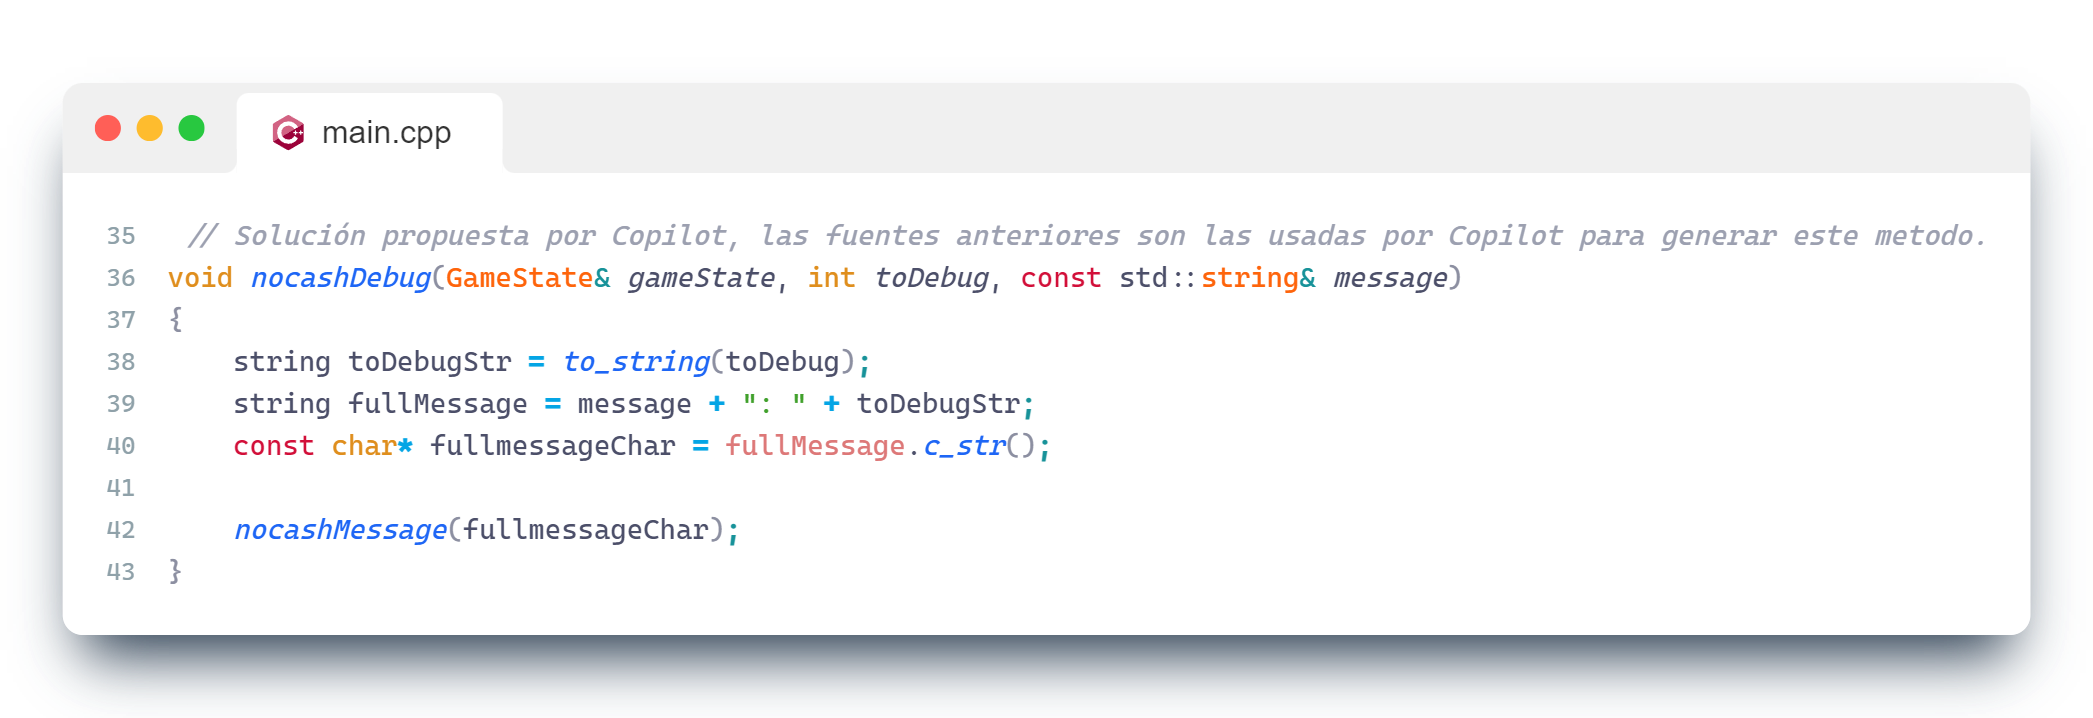
\includegraphics[width=0.75\linewidth]{Imagenes/nocashDebug}
      \caption{Mtodo para sortear nocashMessage()}
      \label{fig:nocashdebug}
    \end{figure}

    Se pasa al mtodo el \texttt{GameState}, un \texttt{int} si hubiese que imprimir una variable, y un mensaje que se convierte a \texttt{string}.

    Primero, se define una variable \texttt{string} y transforma el \texttt{int} a \texttt{string} y luego se concatena en otra variable el texto del parmetro, un par de puntos y luego la variable con el entero convertido. Por ltimo, se define un \texttt{char*} para adaptarlo al \texttt{nocashMessage} y el \texttt{c\textunderscore str()} para convertirlo a \texttt{char*}.

    \begin{figure}[H]
      \centering
      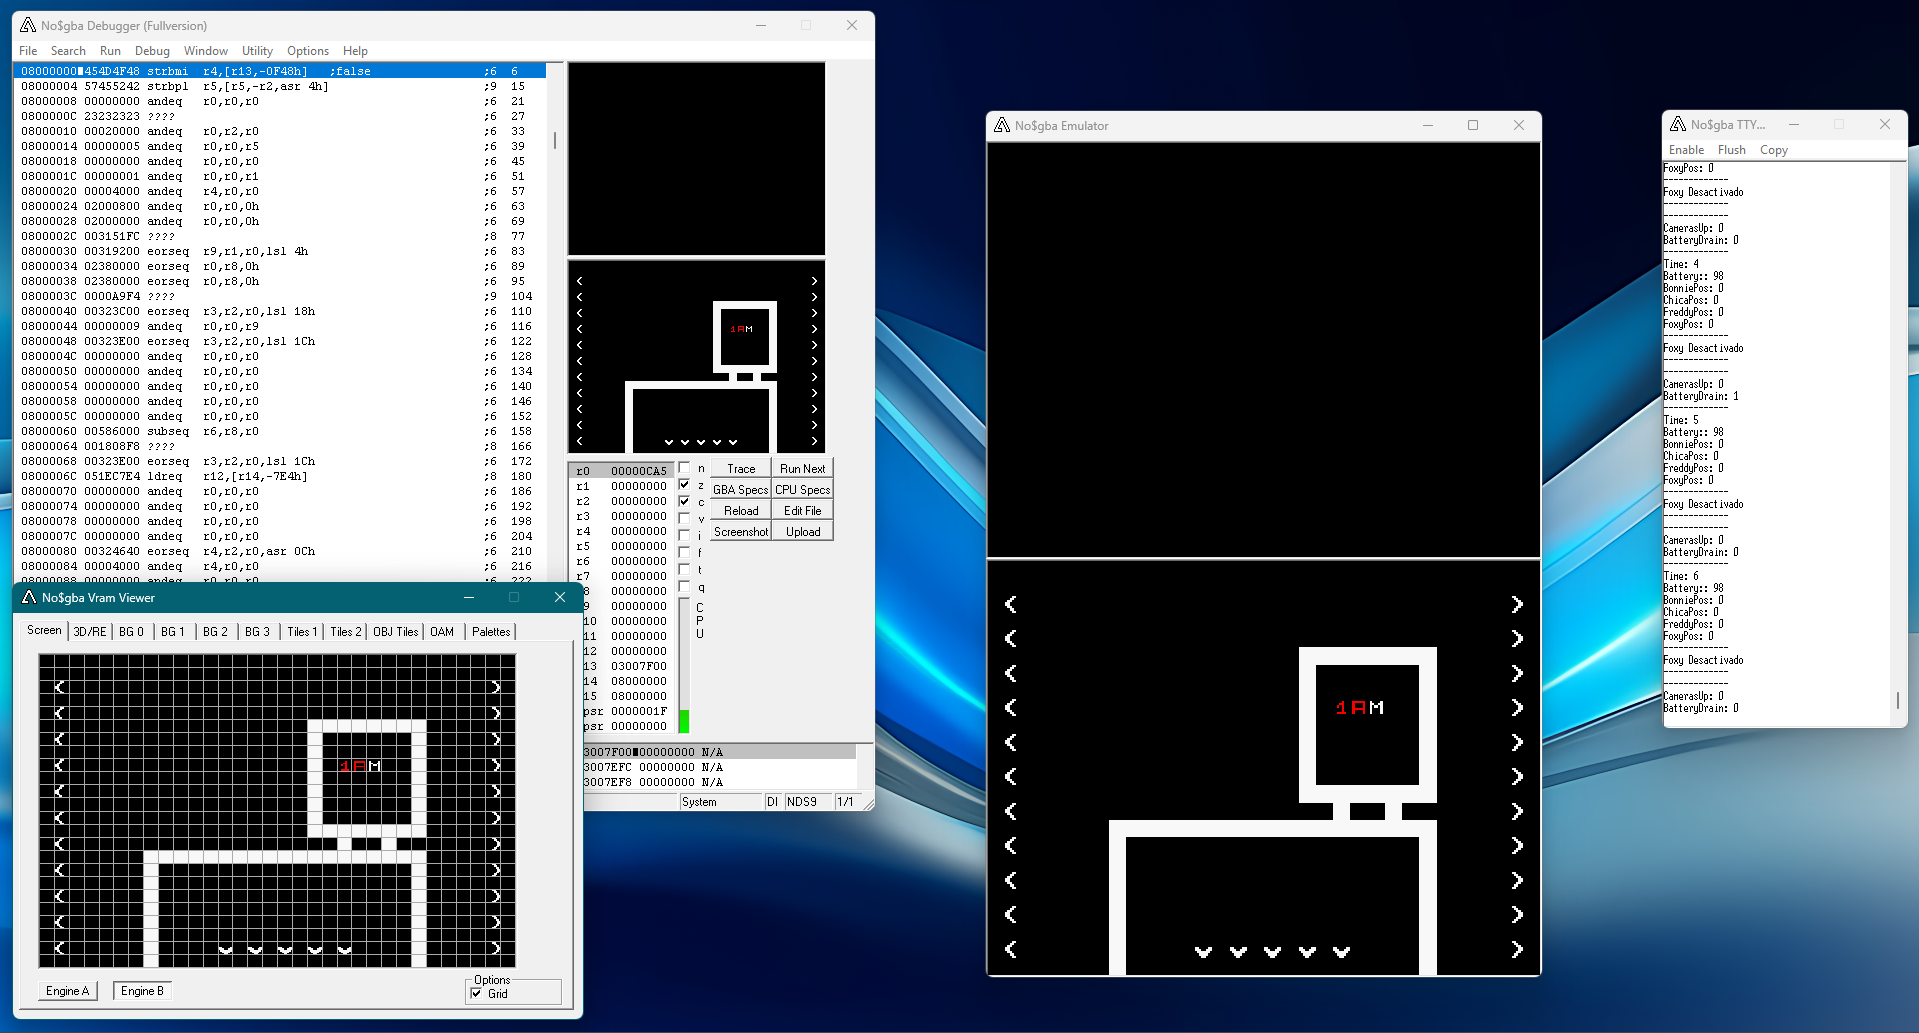
\includegraphics[width=0.75\linewidth]{Imagenes/nocash.png}
      \caption{no\$gba en modo Debug, con ventana de visor de VRAM (izquierda), Debugger (esquina superior izquierda) y consola de depuracin (derecha)}
      \label{fig:nocash}
    \end{figure}


\newpage
\section{Funciones a implementar}
  Numerosas funciones se quedaron en el tintero debido a complicaciones, tiempo, etc. En esta seccin hay una recopilacin del resto de elementos que se quedaron fuera del juego en el momento de entregarlo:

  \begin{enumerate}
    \item \textbf{Freddy}: La IA de Freddy es la ms complicada de todo el juego original, as que se crearon primero los otros enemigos para simplificar el proceso. Sin embargo, la mecnica de Freddy se explica aqu: \ref{freddy}
    \item \textbf{Pulido de Foxy}. La IA de Foxy es la ms complicada de realizar sin contar Freddy, se podra haber pulido el cmo se reinician las interacciones con Foxy, ya que a veces se da la ocasin de que al bloquear correctamente a Foxy, su contador no se reinicie y siga al infinito, efectivamente anulando la amenaza de este.
    \item \textbf{Scroll}. El juego cambia de vistas cambiando totalmente el mapa de teselas, aunque se puede cambiar este mtodo por crear un mapa de teselas mucho ms grande y mientras el jugador mantenga el lpiz en los bordes, se haga scroll por el mapa de teselas ms grande, recreando ms fielmente como funciona el juego original.
    \item \textbf{Sonidos}: Por motivos de tiempo, no se han podido incluir sonidos en la versin final del juego.
    \item \textbf{Animaciones}: Bsicamente, dar ms vida al juego y hacerlo menos esttico; aadir animaciones al abrir y cerrar puertas, Foxy corriendo por las cmaras, etc.
    \item \textbf{Balanceado de dificultad}: Ahora mismo, el juego es relativamente fcil si sabes cmo jugar o Foxy se atasca. Adems, se quera implementar un sistema de dificultad progresiva, en el que segn la noche pase, los enemigos aumenten su nivel de dificultad.
    Esto se puede ver en remanentes del cdigo de los animatrnicos.
  \end{enumerate}

  \paragraph{Freddy \label{freddy} \cite{fnaf_ai}}
  Cuando Freddy supera su \textit{check} de movimiento, activa un temporizador para moverse. Mirar a Freddy en las cmaras para este temporizador, y cambiar har que se reactive.
  Cuando este contador llegue a una cantidad determinada, Freddy se mover.

  Freddy tiene la propiedad de que NO puede ser parado de ninguna manera, y llegar a la esquina de la oficina; y para atacar, la puerta derecha debe estar abierta y no debes estar mirando a Freddy por la cmara, en este caso Freddy fallar todas sus oportunidades de movimiento y la puerta bloquea su paso.

%---------------------------------
%BIBLIOGRAFA
%---------------------------------
\newpage

\printbibliography[title={Bibliografa y agradecimientos}]
\end{document}